% =====================================================================================================================
% Section 6.1, Experiment 1: complete particle-mesh operator action.
% Drop-in replacement for the current Section 6.1. Requires booktabs and graphicx.
% Every number below is generated by ewald_longitudinal/exp1_operator_action.py and exp1_plots.py and is stored in
% exp1_results/summary.json (with the underlying *.csv). Equation numbers in comments refer to draft 3 (asymptotic_check/check_asymptotics.py):
%   split and densities: Eqs. (3), (7)-(13); cutoff tails E_S, E_F: Eq. (17); alias form and mesh law: Eqs. (54), (56), (58).
% Replace the \eqref placeholders in comments by the manuscript labels when merging.
% =====================================================================================================================
\subsection{Experiment 1: complete particle--mesh operator action}
\label{sec:exp1}

Experiment~1 asks whether the operator that the integrator actually applies, $X\mapsto\Gamma_hX$, reproduces the
periodic friction operator $\Gamma$ of the screened longitudinal kernel $K(\mathbf r)=e^{-\kappa r}r^{-1}P(\mathbf r)$,
$\kappa=1$, with the error predicted by the choice of $(\xi,r_c,k_c,h,p)$. We follow the hierarchy used for the
Landau particle method: static configurations first, so that no time-discretization error enters; then each source
of error on its own; then the complete action. The model is not changed for the test. The friction is fully periodic,
the $k=0$ Fourier mode is retained in both the reference and the particle--mesh operator, and there is no free-space
truncation and no energy null space. The only null space is the translation space
$\mathcal T=\mathrm{span}\{T_\alpha\}_{\alpha=1}^3$, $T_\alpha=\mathbf 1_N\otimes\mathbf e_\alpha$.

\paragraph{Why small dense-reference systems.}
Every error in this experiment is measured against a dense $3N\times3N$ matrix $\Gamma_{\rm ref}$ and its full
spectrum. The reference therefore has to be assembled pair by pair over many periodic images, and it has to be
diagonalized. This restricts the experiment to $N\le256$. These sizes are chosen to make the reference computable;
they are not a regime of interest in their own right. The two original test boxes are case~A ($N=30$, $L=6$) and case~B
($N=40$, $L=10$). Here $L$ is the edge length of the periodic cube $[0,L)^3$, not a number of boxes. Their number
densities are $n=N/L^3=0.139$ and $0.040$, and $\kappa L=6$ and $10$. Both are single draws of independent uniform
positions (seeds 7 and 13), with no minimum distance imposed; the closest pairs are at $0.395$ and $0.589$. Case~B was
taken large enough that the smallest nonzero lattice wave number $2\pi/L$ lies below the wave number at which the
longitudinal eigenvalue of $\hat K^L$ changes sign. No physical argument selected $L=6$ for case~A: it is a small box
in which the dense reference is cheap. The parameter sets used later in the paper were accepted when they met their
tolerance on these two boxes. Two boxes are not evidence that the same parameters hold for other configurations, and we
use them only as the starting point.

\paragraph{Configurations.}
Table~\ref{tab:exp1-configs} lists all configurations, including the shortest periodic (minimum-image) pair distance
$d_{\min}$ of each. Since $\kappa=1$, the column $L$ also gives $\kappa L$. The main set has $N=128$ at the density of
case~A, $n_A=30/216$, so $L=9.732$. It contains three families, each with three independent seeds:
\begin{itemize}
\item \emph{uniform}: independent uniform positions with no minimum distance;
\item \emph{perturbed lattice}: a bcc lattice of $4^3$ cells ($N=128$; an fcc lattice of $4^3$ cells for $N=256$),
  every site displaced by an isotropic Gaussian with $\sigma=0.1\,d_{\rm nn}$, plus a random global shift. Here
  $d_{\rm nn}=2.107$ (bcc) or $2.168$ (fcc) is the nearest-neighbour distance;
\item \emph{clustered}: $N/16$ cluster centres drawn uniformly, and 16 particles per cluster drawn from an isotropic
  Gaussian of width $\sigma_c=0.5$ around their centre.
\end{itemize}
For the clustered family, a draw is rejected if it comes closer than $0.25$ to a particle already placed. This avoids
near-coincident pairs, whose $1/r$ kernel would make $\|\Gamma_{\rm ref}\|_2$ arbitrarily large. The realised
$d_{\min}$ is $0.251$--$0.259$ ($N=128$ and $256$), so the constraint is active. For the uniform family, which has no constraint, $d_{\min}$
is $0.142$--$0.411$. One configuration per family at $N=256$ (with $L=12.26$ at the same density) is a smaller
representative check. All random numbers come from seeded generators; the seeds and generator parameters are stored
with the positions.

Two box-length sets are kept apart, because they change different things.
\begin{itemize}
\item In the \emph{fixed-$N$} set, $N=64$ and $L\in\{4,6,8,10,12,16\}$. Changing $L$ therefore also changes the
  density, from $n=1$ to $0.0156$.
\item In the \emph{fixed-density} set, $n=n_A$ and $L\in\{6,8,10,12\}$, so $N=30,71,139,240$.
\end{itemize}
Each set uses three uniform seeds per $L$.

\begin{table}[t]
\centering\small
\caption{Static configurations of Experiment~1. $L$ is the edge length of the periodic cube, $n=N/L^3$ the number
density, $d_{\min}$ the smallest periodic pair distance (range over seeds), $\kappa=1$. A and B are the original two
dense-reference boxes.}
\label{tab:exp1-configs}
\begin{tabular}{llrlllr}
\toprule
set & generation & $N$ & $L=\kappa L$ & $n=N/L^3$ & $d_{\min}$ & seeds \\
\midrule
A & uniform, seed 7 & 30 & 6 & 0.139 & 0.395 & 1 \\
B & uniform, seed 13 & 40 & 10 & 0.040 & 0.589 & 1 \\
U128 & uniform i.i.d. & 128 & 9.73 & 0.139 & 0.142--0.411 & 3 \\
L128 & bcc $4^3$, $\sigma=0.1\,d_{\rm nn}$ & 128 & 9.73 & 0.139 & 1.208--1.366 & 3 \\
C128 & clusters of 16, $\sigma_c=0.5$, $d\ge0.25$ & 128 & 9.73 & 0.139 & 0.251--0.255 & 3 \\
U256 & uniform i.i.d. & 256 & 12.3 & 0.139 & 0.148 & 1 \\
L256 & fcc $4^3$, $\sigma=0.1\,d_{\rm nn}$ & 256 & 12.3 & 0.139 & 1.011 & 1 \\
C256 & clusters of 16, $\sigma_c=0.5$, $d\ge0.25$ & 256 & 12.3 & 0.139 & 0.259 & 1 \\
box-$N$ & uniform i.i.d. & 64 & 4--16 (6 values) & 0.016--1.00 & 0.090--0.723 & 3 \\
box-$n$ & uniform i.i.d. & 30--240 & 6--12 (4 values) & 0.139 & 0.055--0.924 & 3 \\
\bottomrule
\end{tabular}

\end{table}

\paragraph{Reference and its convergence.}
$\Gamma_{\rm ref}$ is built from the unsplit kernel by a direct periodic lattice sum,
\[
(\Gamma_{\rm ref}X)_i=\sum_{j\ne i}\ \sum_{\mathbf m\in\mathbb Z^3,\ |\mathbf r_{ij}+\mathbf mL|\le R}
K(\mathbf r_{ij}+\mathbf mL)\,(X_i-X_j).
\]
It uses neither a minimum-image approximation nor any splitting, and because nothing is removed from the sum the
$k=0$ mode is included automatically. The image radius was increased through
$R=15,20,\dots,45$. Over all 44 configurations, the largest change relative to $R=45$ is $2.5\times10^{-12}$ at
$R=30$, $2.0\times10^{-14}$ at $R=35$, and $4.3\times10^{-16}$ at $R=40$, measured in $\|\cdot\|_2/\|\Gamma_{\rm ref}\|_2$.
This change follows the tail $e^{-\kappa R}$ until it reaches round-off. We take $R=45$ as the reference. The ladder
shares its inner shells, so it bounds only the image truncation, which is below $10^{-15}$. Round-off in the common
sum is checked independently by the split construction below, which reproduces $\Gamma_{\rm ref}$ to
$6.7\times10^{-15}$--$2.2\times10^{-13}$. Both levels are far below the smallest approximation error measured against
the reference in this section, $2.3\times10^{-10}$. The reference is symmetric to $1.0\times10^{-16}$ and annihilates
the translations to $1.9\times10^{-16}$, both relative.

\paragraph{Split identity and coefficient accuracy.}
On nonzero separations, $\theta_S$ is evaluated in closed form and $\theta_L$ from its own $s$-integral (not as
$e^{-\kappa r}/r-\theta_S$). The identity $\theta_S+\theta_L=e^{-\kappa r}/r$ (draft Eqs.~(7)--(8)) then holds to
$2.5\times10^{-15}$ relative error. This was checked for $\xi\in\{0.5,0.7,1,1.4,2\}$, on a radial grid
$10^{-3}\le r\le20$, and on every pair image with $r\le12$ of the main and legacy configurations.

At operator level we combine two independent constructions:
\begin{itemize}
\item $\Gamma_S$ from the real-space lattice sum of $\theta_S$ over $|\mathbf r+\mathbf mL|\le45$;
\item $\Gamma_L^{\rm F}$ from the untruncated (mesh-free) lattice Fourier sum
  $V^{-1}\sum_{|\mathbf k|\le k_c}\hat K^L(\mathbf k)\cos(\mathbf k\cdot\mathbf r)$, with $k_c=2\xi\cdot6.5$
  ($e^{-(k_c/2\xi)^2}\approx2\times10^{-19}$), including $\mathbf k=0$.
\end{itemize}
Their sum reproduces $\Gamma_{\rm ref}$ to between $6.7\times10^{-15}$ and $2.2\times10^{-13}$
(Fig.~\ref{fig:exp1-components}a). The largest values occur for the perturbed lattices, whose $\|\Gamma_{\rm ref}\|_2$ is
smallest. The same level is the plateau of the Fourier-cutoff sweep below, and it grows with the number of retained
modes. It therefore belongs to the float64 comparison of a Fourier lattice sum with a real-space lattice sum, not to the
split identity, which holds pointwise to $2.5\times10^{-15}$. A recorded check (case~A, a perturbed lattice and a uniform
configuration at $\xi=0.7$ and $1$) narrows this down. The floor ($2.3\times10^{-14}$--$1.5\times10^{-13}$) agrees to
within $0.2\%$ across three variants: float64 accumulation, 80-bit accumulation of the same inputs, and coefficients from
the refined quadrature rules. The float64 and 80-bit sums differ by at most $7\times10^{-16}$. The floor is therefore
set neither by the accumulation nor by the coefficient quadrature. Its remaining sources, the rounding of positions and
wave vectors in the phases $\mathbf k\cdot\mathbf r$ and the real-space sum $\Gamma_L$ it is compared with, were not
separated.
The coefficients themselves are accurate. With the Gauss--Legendre rules for $A(k)$, $B(k)$ and $\theta_L$ refined (twice
the panels, 30 nodes per panel), these change by at most $1.6\times10^{-15}$, relative to $\|\hat K^L(k)\|_2$ or to
$e^{-\kappa r}/r$, for $\xi\le2$, $k\le14\xi$ and $10^{-3}\le r\le20$. The quadrature of $\theta_S$ agrees with its closed
form to $1.0\times10^{-15}$.

\paragraph{Real-space and Fourier cutoffs.}
Each truncation is measured with no other approximation present:
\begin{itemize}
\item $\|\Gamma_S^{r_c}-\Gamma_S\|_2$, where $\Gamma_S$ is the real-space lattice sum of $\theta_S$ over
  $|\mathbf r+\mathbf mL|\le45$;
\item $\|\Gamma_L^{k_c}-\Gamma_L\|_2$, where $\Gamma_L^{k_c}$ is the mesh-free lattice Fourier sum over
  $|\mathbf k|\le k_c$, and $\Gamma_L$ is the real-space lattice sum of $\theta_L$ over $|\mathbf r+\mathbf mL|\le45$
  ($\theta_L=e^{-\kappa r}/r-\theta_S$ for $\xi r\ge1.5$, its $s$-integral otherwise).
\end{itemize}
Both are normalized by $\|\Gamma_{\rm ref}\|_2$ (Fig.~\ref{fig:exp1-components}b,c). We fit $\log E=a-cx^2$ with
$x=\xi r_c$ or $x=k_c/(2\xi)$, using only $x\ge1$ and $E\ge10^{-12}$, so that any round-off plateau is excluded. Steps
at which a larger cutoff admits no new pair image or lattice shell are left out of the fit (see below).

At $\xi=0.7$ the fitted Gaussian rates are:
\begin{itemize}
\item real space: median $c=0.99$, range $0.98$--$1.03$ over the eleven main and legacy configurations;
\item Fourier space: median $c=0.97$, range $0.96$--$1.00$.
\end{itemize}
At $\xi=1$ the medians are again $0.99$ (range $0.98$--$1.03$) and $0.97$ ($0.96$--$1.00$). The $N=256$ configurations
fall in the same ranges. Removing the continuum prefactor of the tails (draft Eq.~(17), $E\propto x\,e^{-x^2}$) by
dividing by $x$ overcorrects, giving medians of $1.05$ (real space) and $1.03$ (Fourier). Neither form gives $c=1$
within the fit window, so the algebraic prefactor of the operator-norm error is not that of the continuum tail. We do
not interpret $c$ as a measured universal exponent.

The real-space error is still decreasing at the largest cutoff, $\xi r_c=6.5$, where it is at most
$9\times10^{-17}$; only three of the 28 curves level off near $10^{-16}$. The Fourier error reaches a plateau of
$1.2\times10^{-13}$ ($\xi=0.7$) and $1.6\times10^{-13}$ ($\xi=1$) in every configuration: this is the lattice-sum floor
discussed above. The finite particle set makes the curves staircases at small cutoffs:
\begin{itemize}
\item on the perturbed lattices, 13 real-space steps with $\xi r_c\le1.25$ admit no new pair image;
\item for case~A, 3 Fourier steps with $k_c/(2\xi)\le1$ admit no new lattice shell.
\end{itemize}
These points keep their equal errors and are flagged in the data, not smoothed. The seven of them that fall inside a
fit window are excluded from the fits.

\paragraph{Mesh spacing, B-spline order and aliasing.}
With $\xi=0.7$ and the production Fourier cutoff $k_c=5.74$ ($s=4.1$), we compare the particle--mesh long-range
operator with the mesh-free lattice sum over the same modes. The difference $\Gamma_L^{\rm mesh}-\Gamma_L^{k_c}$ is then
pure mesh error, with no truncation in it. For the eleven main and legacy configurations the scan covers $p=3,\dots,8$
and nine FFT-friendly meshes from $\eta=k_ch/\pi\approx0.91$--$0.99$ down to $0.23$--$0.25$. Each mesh is evaluated at
eight grid shifts: the unshifted grid and seven random global offsets in $[0,h)^3$ (Fig.~\ref{fig:exp1-components}d--f).
The $N=256$ checks use $p=5,7$, six meshes ($\eta$ down to $0.23$) and four shifts. The scan was repeated at a converged
cutoff, $s=5.5$ ($e^{-s^2}\approx7\times10^{-14}$), for $p=4,6,8$, seven meshes and eight shifts, on cases A and B and
seed~1 of each $N=128$ family. Adjacent meshes differ by 7--41\% in $h$.

We fit the RMS over shifts on the four finest meshes with error at least $10^{-12}$. The threshold excludes meshes
on which the error approaches the $\sim10^{-13}$ floor of the Fourier lattice sum it is compared with: the finest
meshes for $p=8$ at $s=5.5$ (the error falls to $8.9\times10^{-14}$ at $\eta=0.25$), and at $s=4.1$ the finest mesh for
one configuration (uniform, seed~3) at $p=8$. At $s=4.1$ the fit windows therefore lie between $\eta=0.23$ and
$0.50$, typically $0.25$--$0.40$; at $s=5.5$ they reach up to $\eta=0.77$. The fitted slopes in $h$ are, as medians
with ranges over the eleven main and legacy configurations ($s=4.1$) and over the five configurations of the $s=5.5$
scan:

\begin{center}\small
\begin{tabular}{ccc}
\toprule
$p$ & slope at $s=4.1$, median (range) & slope at $s=5.5$, median\\
\midrule
3 & 3.09 (2.90--3.22) & --\\
4 & 4.07 (3.85--4.36) & 4.10\\
5 & 5.24 (4.88--5.43) & --\\
6 & 6.19 (6.13--6.44) & 6.25\\
7 & 7.46 (7.03--7.66) & --\\
8 & 8.50 (8.42--8.88) & 8.87\\
\bottomrule
\end{tabular}
\end{center}

For $p=5,7$ the three $N=256$ checks give $5.12$--$5.39$ and $7.44$--$7.58$, inside these ranges. In the fitted
windows the error is therefore $O(h^p)$ for every family. The median slopes exceed $p$ for $p\ge5$, by up to $1.0$
for $p=8$ (one $p=5$ fit is $4.88$). On the coarse meshes ($\eta=0.55$--$0.99$) the decay is clearly faster than $h^p$:
the median exponents there are $3.31$, $4.53$, $5.97$, $7.30$, $8.68$ and $10.18$ for $p=3,\dots,8$, or $1.10$--$1.27\,p$.
Both observations are consistent with the leading alias image (draft Eqs.~(54),~(58)). Its factor $q^p$, with
$q=\eta_k/(2-\eta_k)$ and $\eta_k=kh/\pi\le\eta$ for a retained mode $k$, has local exponent between $p$ and $2p/(2-\eta)$
in $h$, and reaches $p$ only as $\eta\to0$. Slopes between adjacent meshes are too noisy to show this directly. The
$h^p$ law is thus observed for $\eta\approx0.23$--$0.50$; its asymptotic constant has not been reached, and we report no
such constant.

The phase sensitivity is moderate. Over all eight-shift scans, the largest error over shifts is at most $1.30$ times
the RMS and at most $1.92$ times the smallest. Fitted on the same windows, the slope of the maximum differs from that of
the RMS by $-0.26$ to $+0.20$. On the unshifted grid, the complete off-grid decomposition
\[
K_h-K_F=V^{-1}\sum_{\mathbf k}e^{i\mathbf k\cdot\mathbf r_{ij}}\bigl[D_h+H_h(\alpha_i^*+\alpha_j+\alpha_i^*\alpha_j)\bigr]
\]
reproduces the particle--mesh pair response to $3\times10^{-15}$ of $\max|K_F|$. The literal spread--FFT--influence--gather
response, computed one source particle at a time, agrees with the mode-space pair response to $1.3\times10^{-15}$. We
checked this for $p=4,7$ on two meshes for case~A, case~B and seed~1 of each $N=128$ family. In the decomposition:
\begin{itemize}
\item the linear cross terms $\alpha_i^*+\alpha_j$ between the principal term and the aliases carry $0.996$--$1.003$ of
  the mesh error (spectral norm);
\item the alias--alias term carries at most $0.9\%$;
\item $D_h$ vanishes to $5\times10^{-9}$ of the error, as it should with ideal deconvolution.
\end{itemize}
An estimate that kept only the alias--alias term would therefore miss the mesh error almost completely.

\paragraph{The complete production action.}
We now apply the production code path itself: the real-space pair loop, B-spline spreading of the three components,
FFT, multiplication by the influence function $\hat K^L/|\hat W|^2$ on $|\mathbf k|\le k_c$, inverse FFT, adjoint
gather, and the degree correction. We use it in two ways:
\begin{itemize}
\item applied to the $3N$ unit vectors, it gives $\Gamma_h$ column by column, without any hand-assembled matrix;
\item applied to probe vectors, it gives the action directly.
\end{itemize}
Three parameter sets were tested (Table~\ref{tab:exp1-params}): the cheapest sets accepted at $\xi=0.7$ for the
tolerances $10^{-5}$, $10^{-7}$ and $10^{-9}$ on cases A and B (T5, T7, T9). The literal columns agree with an
independent mode-space assembly to $1.1\times10^{-15}$. That assembly, in turn, equals an independently built
real-space cutoff sum $\Gamma_S^{r_c}$ plus the same mesh pair matrix $\Gamma_L^{\rm mesh}$ to $1.4\times10^{-15}$. The
budget terms $\varepsilon_S=\|\Gamma_S^{r_c}-\Gamma_S\|_2$, $\varepsilon_F=\|\Gamma_L^{k_c}-\Gamma_L\|_2$ and
$\varepsilon_{\rm mesh}=\|\Gamma_L^{\rm mesh}-\Gamma_L^{k_c}\|_2$, all normalized by $\|\Gamma_{\rm ref}\|_2$, therefore
telescope to the production error. All three sets keep $\mathbf k=0$ and exclude no influence mode.

\begin{table}[t]
\centering\small
\caption{Parameter sets of the production action test (accepted at $\xi=0.7$ for the stated tolerance on cases A and
B). $M$ is the next $2,3,5$-smooth mesh size with $h\le\eta_N\pi/k_c$; the realised $\eta=k_ch/\pi$ is therefore at most
$\eta_N$ and depends on $L$.}
\label{tab:exp1-params}
\begin{tabular}{lllllll}
\toprule
set & $\xi$ & $s$ & $r_c=s/\xi$ & $k_c=2\xi s$ & $\eta_N$, $p$ & $M$ (A / B / $N\!=\!128$ / $N\!=\!256$) \\
\midrule
T5 & 0.7 & 3.494 & 4.991 & 4.891 & 0.8, 6 & 12 / 20 / 20 / 24 \\
T7 & 0.7 & 4.100 & 5.857 & 5.740 & 0.7, 7 & 16 / 27 / 27 / 36 \\
T9 & 0.7 & 4.628 & 6.611 & 6.479 & 0.6, 8 & 24 / 36 / 36 / 45 \\
\bottomrule
\end{tabular}

\end{table}

Figure~\ref{fig:exp1-action}a shows the relative spectral error $\|\Gamma_h-\Gamma_{\rm ref}\|_2/\|\Gamma_{\rm
ref}\|_2$. Cases A and B meet their tolerances, as they were selected to. The uniform and clustered configurations at
$N=128$ and $256$ meet them with margin. The perturbed lattices do not:
\begin{itemize}
\item T5: $1.16$--$1.29\times10^{-5}$;
\item T7: $1.94$--$2.11\times10^{-7}$ at $N=128$ and $1.09\times10^{-7}$ at $N=256$;
\item T9: $1.96$--$2.55\times10^{-9}$.
\end{itemize}
The excess is up to a factor $2.6$.

Figure~\ref{fig:exp1-action}b shows the reason. At T7, the absolute error $\|\Gamma_h-\Gamma_{\rm ref}\|_2$ lies in
$5.7\times10^{-8}$--$5.5\times10^{-7}$ over all 44 configurations, a spread below a factor ten. It still depends
systematically on the configuration: it is $3.4$--$5.2\times10^{-7}$ for the clustered and $1.0$--$1.5\times10^{-7}$ for
the perturbed-lattice configurations, and it grows with density (see below). Meanwhile $\|\Gamma_{\rm ref}\|_2$ ranges
from $0.72$ to $35$, set by the closest pairs through $\theta(d_{\min})\approx e^{-d_{\min}}/d_{\min}$. Perturbed lattices
have no pair closer than $1.0$ and the smallest norms ($0.72$--$0.94$). A tolerance stated relative to $\|\Gamma_{\rm
ref}\|_2$ and calibrated on configurations that contain close pairs therefore does not transfer to configurations without
them: the absolute error varies far less than the relative one, which inherits the configuration dependence of the norm.

For the main and legacy configurations at T7 the mesh term is the largest in the budget ($\le1.5\times10^{-7}$
relative), followed by the real-space and Fourier truncations ($\le1.0\times10^{-7}$ and $\le7\times10^{-8}$, largest for
the lattices). The real-space term is comparable or larger for the $N=256$ lattice and for the boxes with the smallest
realised $\eta$ (fixed-$N$ $L=4$, fixed-density $L=8$), and at T5 it is the largest for the uniform and lattice
configurations.

The probes are applied through the production matvec (Fig.~\ref{fig:exp1-action}c):
\begin{itemize}
\item sixteen mean-free Gaussian vectors;
\item the lowest nonzero periodic wave number $2\pi/L$ along each axis, longitudinal and transverse, cosine and sine,
  projected onto $\mathcal T^\perp$;
\item the three translations.
\end{itemize}
At T7 the largest relative action errors $\|(\Gamma_h-\Gamma_{\rm ref})X\|/\|\Gamma_{\rm ref}X\|$ on the main and legacy
sets are $1.7\times10^{-7}$ (Gaussian), $2.7\times10^{-7}$ (longitudinal) and $4.2\times10^{-7}$ (transverse), against a
largest relative spectral error of $2.1\times10^{-7}$. A relative action error can exceed the configuration's own relative
spectral error by at most the factor $\|\Gamma_{\rm ref}\|_2\|X\|/\|\Gamma_{\rm ref}X\|$. For the long-wavelength modes,
which lie close to the null space of the graph Laplacian, this factor is large: $\|\Gamma_{\rm ref}X\|/(\|\Gamma_{\rm
ref}\|_2\|X\|)$ is as small as $2.5\times10^{-2}$ (longitudinal) and $1.1\times10^{-2}$ (transverse) on the main and
legacy sets. Every longitudinal and transverse probe exceeds its configuration's relative spectral error, by up to a factor
$14$ and $18$. Only about half of the Gaussian probes do, by up to a factor $6$. On the perturbed lattices, whose spectral
error is largest, the Gaussian errors stay below it. The box-length sets reach smaller ratios ($6.5\times10^{-3}$ and
$2.9\times10^{-3}$, for a configuration with a pair at $0.055$ and $\|\Gamma_{\rm ref}\|_2=35$), with correspondingly larger
factors. For the translations we report operator-normalized residuals instead of dividing by a zero reference action:
\begin{itemize}
\item the production $\Gamma_hT_\alpha$ is exactly zero in floating point, because the degree correction cancels the
  constant field term by term;
\item $\|\Gamma_{\rm ref}T_\alpha\|/(\|\Gamma_{\rm ref}\|_2\|T_\alpha\|)\le1.9\times10^{-16}$.
\end{itemize}
The literal $\Gamma_h$ is symmetric to $1.0\times10^{-16}$ (relative Frobenius norm). For Experiment~3 we record the
smallest eigenvalue on $\mathcal T^\perp$. It ranges over $8\times10^{-4}$--$1.92$ across the configurations, and is
changed by $\Gamma_h$ by at most $4.2\times10^{-5}$ (T5), $1.6\times10^{-6}$ (T7) and $2.6\times10^{-8}$ (T9) relative.
In every case $\|\Gamma_h-\Gamma_{\rm ref}\|_2<\lambda_{\min}(\Gamma_{\rm ref}|_{\mathcal T^\perp})$, with margin at least
$0.997\,\lambda_{\min}$.

\paragraph{Box length.}
At T7, the two box-length sets give different information (Fig.~\ref{fig:exp1-action}d).

All values below are medians over the three seeds.

At fixed $N=64$ the density changes with $L$. The absolute error falls from $5.3\times10^{-7}$ ($L=4$, $n=1$) to
$1.0\times10^{-7}$ ($L=16$, $n=0.016$). All three budget terms fall with the density:
\begin{itemize}
\item the absolute real-space term goes from $3.2\times10^{-7}$ to $2.6\times10^{-8}$ (sublinear in $n$);
\item the Fourier term goes from $1.2\times10^{-7}$ to $1.8\times10^{-8}$;
\item the mesh term goes from $2.9\times10^{-7}$ to $8.8\times10^{-8}$; it is the largest term for $L\ge6$, and it is also
  modulated by the realised $\eta$.
\end{itemize}
Rounding $M$ to a $2,3,5$-smooth size gives $\eta=0.61$ at $L=4$ and $8$ but $0.65$--$0.69$ otherwise. This rounding
causes the dip at $L=8$.

At fixed density $n_A$ the absolute error is $2.1\times10^{-7}$ ($L=6$), $1.1\times10^{-7}$ ($L=8$, $\eta=0.61$),
$2.5\times10^{-7}$ ($L=10$) and $2.5\times10^{-7}$ ($L=12$). The dip at $L=8$ is again the mesh rounding. At nearly equal
$\eta$ ($0.68$--$0.69$), $L=10$ and $12$ lie about $20\%$ above $L=6$, beyond the seed spread
($2.0$--$2.1\times10^{-7}$ against $2.3$--$2.7\times10^{-7}$), mostly in the mesh term ($1.9$ against
$2.3\times10^{-7}$). We did not isolate the cause of this residual $L$ dependence.

A fixed-$N$ comparison is therefore mainly a density test. Only the fixed-density comparison isolates $L$, and over
$L=6$--$12$ it shows changes of at most a factor $2.2$, dominated by the realised $\eta$. The relative error additionally
inherits the configuration-dependent $\|\Gamma_{\rm ref}\|_2$, as above.

\paragraph{What the experiment supports.}
The original cases A and B show that the accepted parameter sets meet their relative tolerances on two uniform boxes.
On their own they do not support a claim about other configurations. The supplementary experiment adds the following:
\begin{enumerate}
\item an independent reference built from the unsplit kernel, with $k=0$, whose image truncation converges to below
  $10^{-15}$ and which an independent split construction reproduces to $\le2.2\times10^{-13}$;
\item the split identity and the coefficient quadrature at round-off over a range of $\xi$;
\item the Gaussian decay of both truncations and the $O(h^p)$ mesh law on $\eta\approx0.23$--$0.50$, with consistent
  rates across three configuration families, two particle numbers and grid shifts, and with the linear alias cross terms
  identified as the mesh error;
\item a verification of the production spread--FFT--influence--gather action itself, including null-space and symmetry
  properties.
\end{enumerate}
It also shows a limitation of the original acceptance: tolerances defined relative to $\|\Gamma_{\rm ref}\|_2$ are
configuration dependent and are exceeded by up to a factor $2.6$ on perturbed lattices. The absolute error varies by less
than a factor ten across all configurations, with a systematic dependence on clustering and density, far less than the
relative error does. Parameter selection for production runs should therefore be calibrated on the configuration class
with the smallest $\|\Gamma\|_2$, or on an absolute scale.

All results are for $\kappa=1$, $N\le256$ and static configurations. The $h^p$ rate is observed for
$\eta\approx0.23$--$0.50$; on coarser meshes the decay is faster ($1.1$--$1.3\,p$), and the asymptotic constant of the law
was not reached.

\begin{figure}[t]
\centering
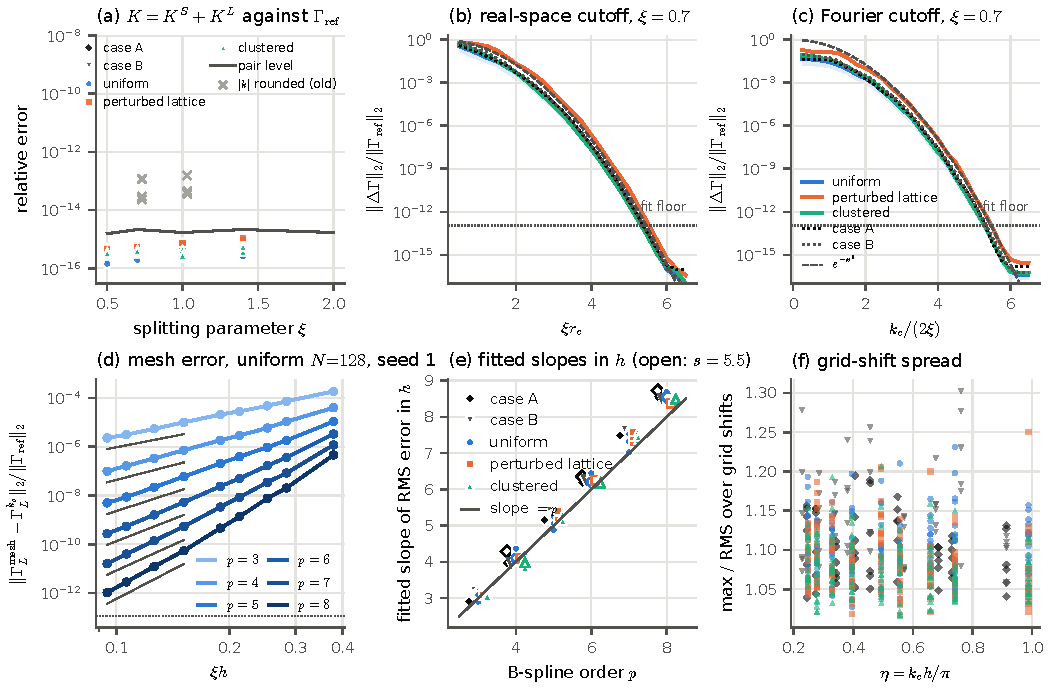
\includegraphics[width=\textwidth]{figures/exp1_components.pdf}
\caption{Error sources of Experiment~1, $\kappa=1$.
(a)~Split identity: $\Gamma_S$ (real-space lattice sum) plus $\Gamma_L^{\rm F}$ (mesh-free lattice Fourier sum,
$k_c=2\xi\cdot6.5$) against $\Gamma_{\rm ref}$. The line is the pair-level error $\max_r|\theta_S+\theta_L-e^{-\kappa r}/r|/(e^{-\kappa r}/r)$.
(b)~Real-space and (c)~Fourier truncation at $\xi=0.7$, with no other approximation present. The curves are the median over three
seeds and the band is their range; dotted curves are cases A and B; the dashed curve is $e^{-x^2}$.
(d)~Mesh error against the mesh-free lattice sum over the same modes at the production $k_c=5.74$, for uniform $N=128$,
seed~1. The curves are the RMS over eight grid shifts, the bands the range over shifts, and the thin segments have slope
$p$.
(e)~Fitted slopes in $h$ on the four finest meshes with error $\ge10^{-12}$. Filled markers use the production $k_c$; open
markers use $k_c$ at $s=5.5$ (five configurations).
(f)~Largest over RMS error across the eight grid shifts, for every mesh and $p$ of the eight-shift scans ($N\le128$,
production $k_c$).}
\label{fig:exp1-components}
\end{figure}

\begin{figure}[t]
\centering
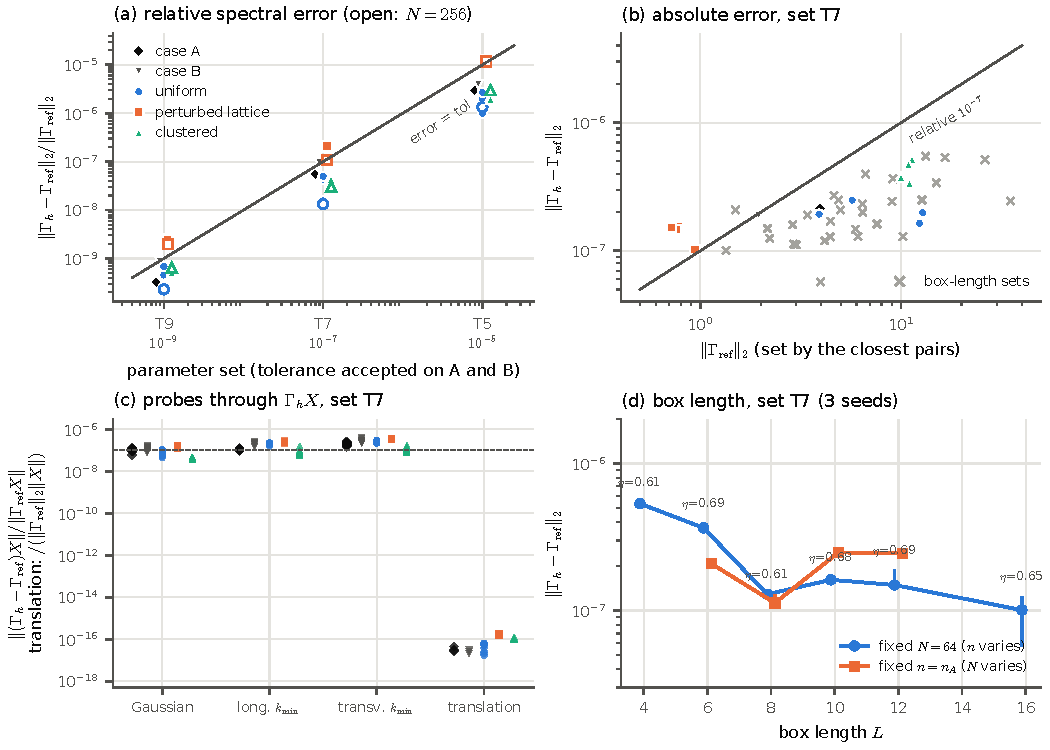
\includegraphics[width=\textwidth]{figures/exp1_action.pdf}
\caption{The production action $X\mapsto\Gamma_hX$ against the dense full-periodic reference.
(a)~Relative spectral error for the parameter sets accepted at $10^{-9}$, $10^{-7}$ and $10^{-5}$ on cases A and B.
Filled markers are $N\le128$ and open markers $N=256$.
(b)~Absolute error against $\|\Gamma_{\rm ref}\|_2$ at T7; the diagonal is relative $10^{-7}$; crosses are the box-length
sets.
(c)~Probe errors through the production matvec at T7. Translations are given as operator-normalized residuals; the dashed
line is $10^{-7}$.
(d)~Absolute error against box length at T7, at fixed $N=64$ (density varies) and at fixed density $n_A$ ($N$ varies).
The realised $\eta$ is annotated.}
\label{fig:exp1-action}
\end{figure}
